\section{Introduction}
Despite the well-recognized importance of training data in advancing the capabilities of large language models (LLMs)~\cite{brown2020language,kaplan2020scaling,Razeghi2022ImpactOP}, there is no agreed-upon mechanisms for crediting or compensating data providers. As LLMs are increasingly integrated into our society and economy, the absence of such mechanisms has aggravated a tension between data and model providers, exemplified by recent legal challenges involving major tech companies~\cite{jlversusalphabet,metz2022lawsuit}. In this atmosphere, data valuation, which quantifies the contribution of each training data to the model output, has been discussed as a potential technical solution for tackling these societal issues~\cite{fernandez2023data,ghorbani2019data,huang2023citation,jia2019towards,worledge2023unifying,zhao2023addressing}. 

At a high level, most data valuation algorithms interpret the model output as a coalition of its training data, and evaluate the contribution of each example based on its influence on the model output when included or excluded from the training dataset~\cite{ghorbani2019data,ilyas2022datamodels,koh2017understanding,kwon2021beta}. If an inclusion of a specific training example consistently improves model performance, high value can be assigned to this example for its contribution. However, applying existing data valuation methods to recent LLMs and their vast training datasets has faced significant scalability challenges to date. For instance, sampling-based methods, such as the Shapley value~\cite{ghorbani2019data,kwon2021beta} or Datamodels~\cite{ilyas2022datamodels}, require retraining the model multiple times with varied combinations of data subsets to directly model the effect of in/excluding each data. Unfortunately, such repeated retraining is hardly affordable even for small models, let alone LLMs. To overcome this issue, gradient-based methods, including influence functions~\cite{koh2017understanding,park2023trak}, approximate the effect of data in/exclusion on the model output using gradient information without costly retraining. Even so, scaling gradient-based methods to LLMs is hindered by prohibitive compute and memory costs originating in the high-dimensional nature of the gradient.

Consequently, the main objective of this work is to bridge the gap in scaling existing data valuation methods to recent LLMs and their vast training datasets. Toward this goal, we focus on influence functions \cite{koh2017understanding,park2023trak}, a representative gradient-based data valuation method, and significantly improve its scalability with an efficient gradient projection algorithm. We visualize the proposed data valuation system in Figure~\ref{fig:diagram}, and detail our technical contributions below:

\begin{figure}
    \centering
    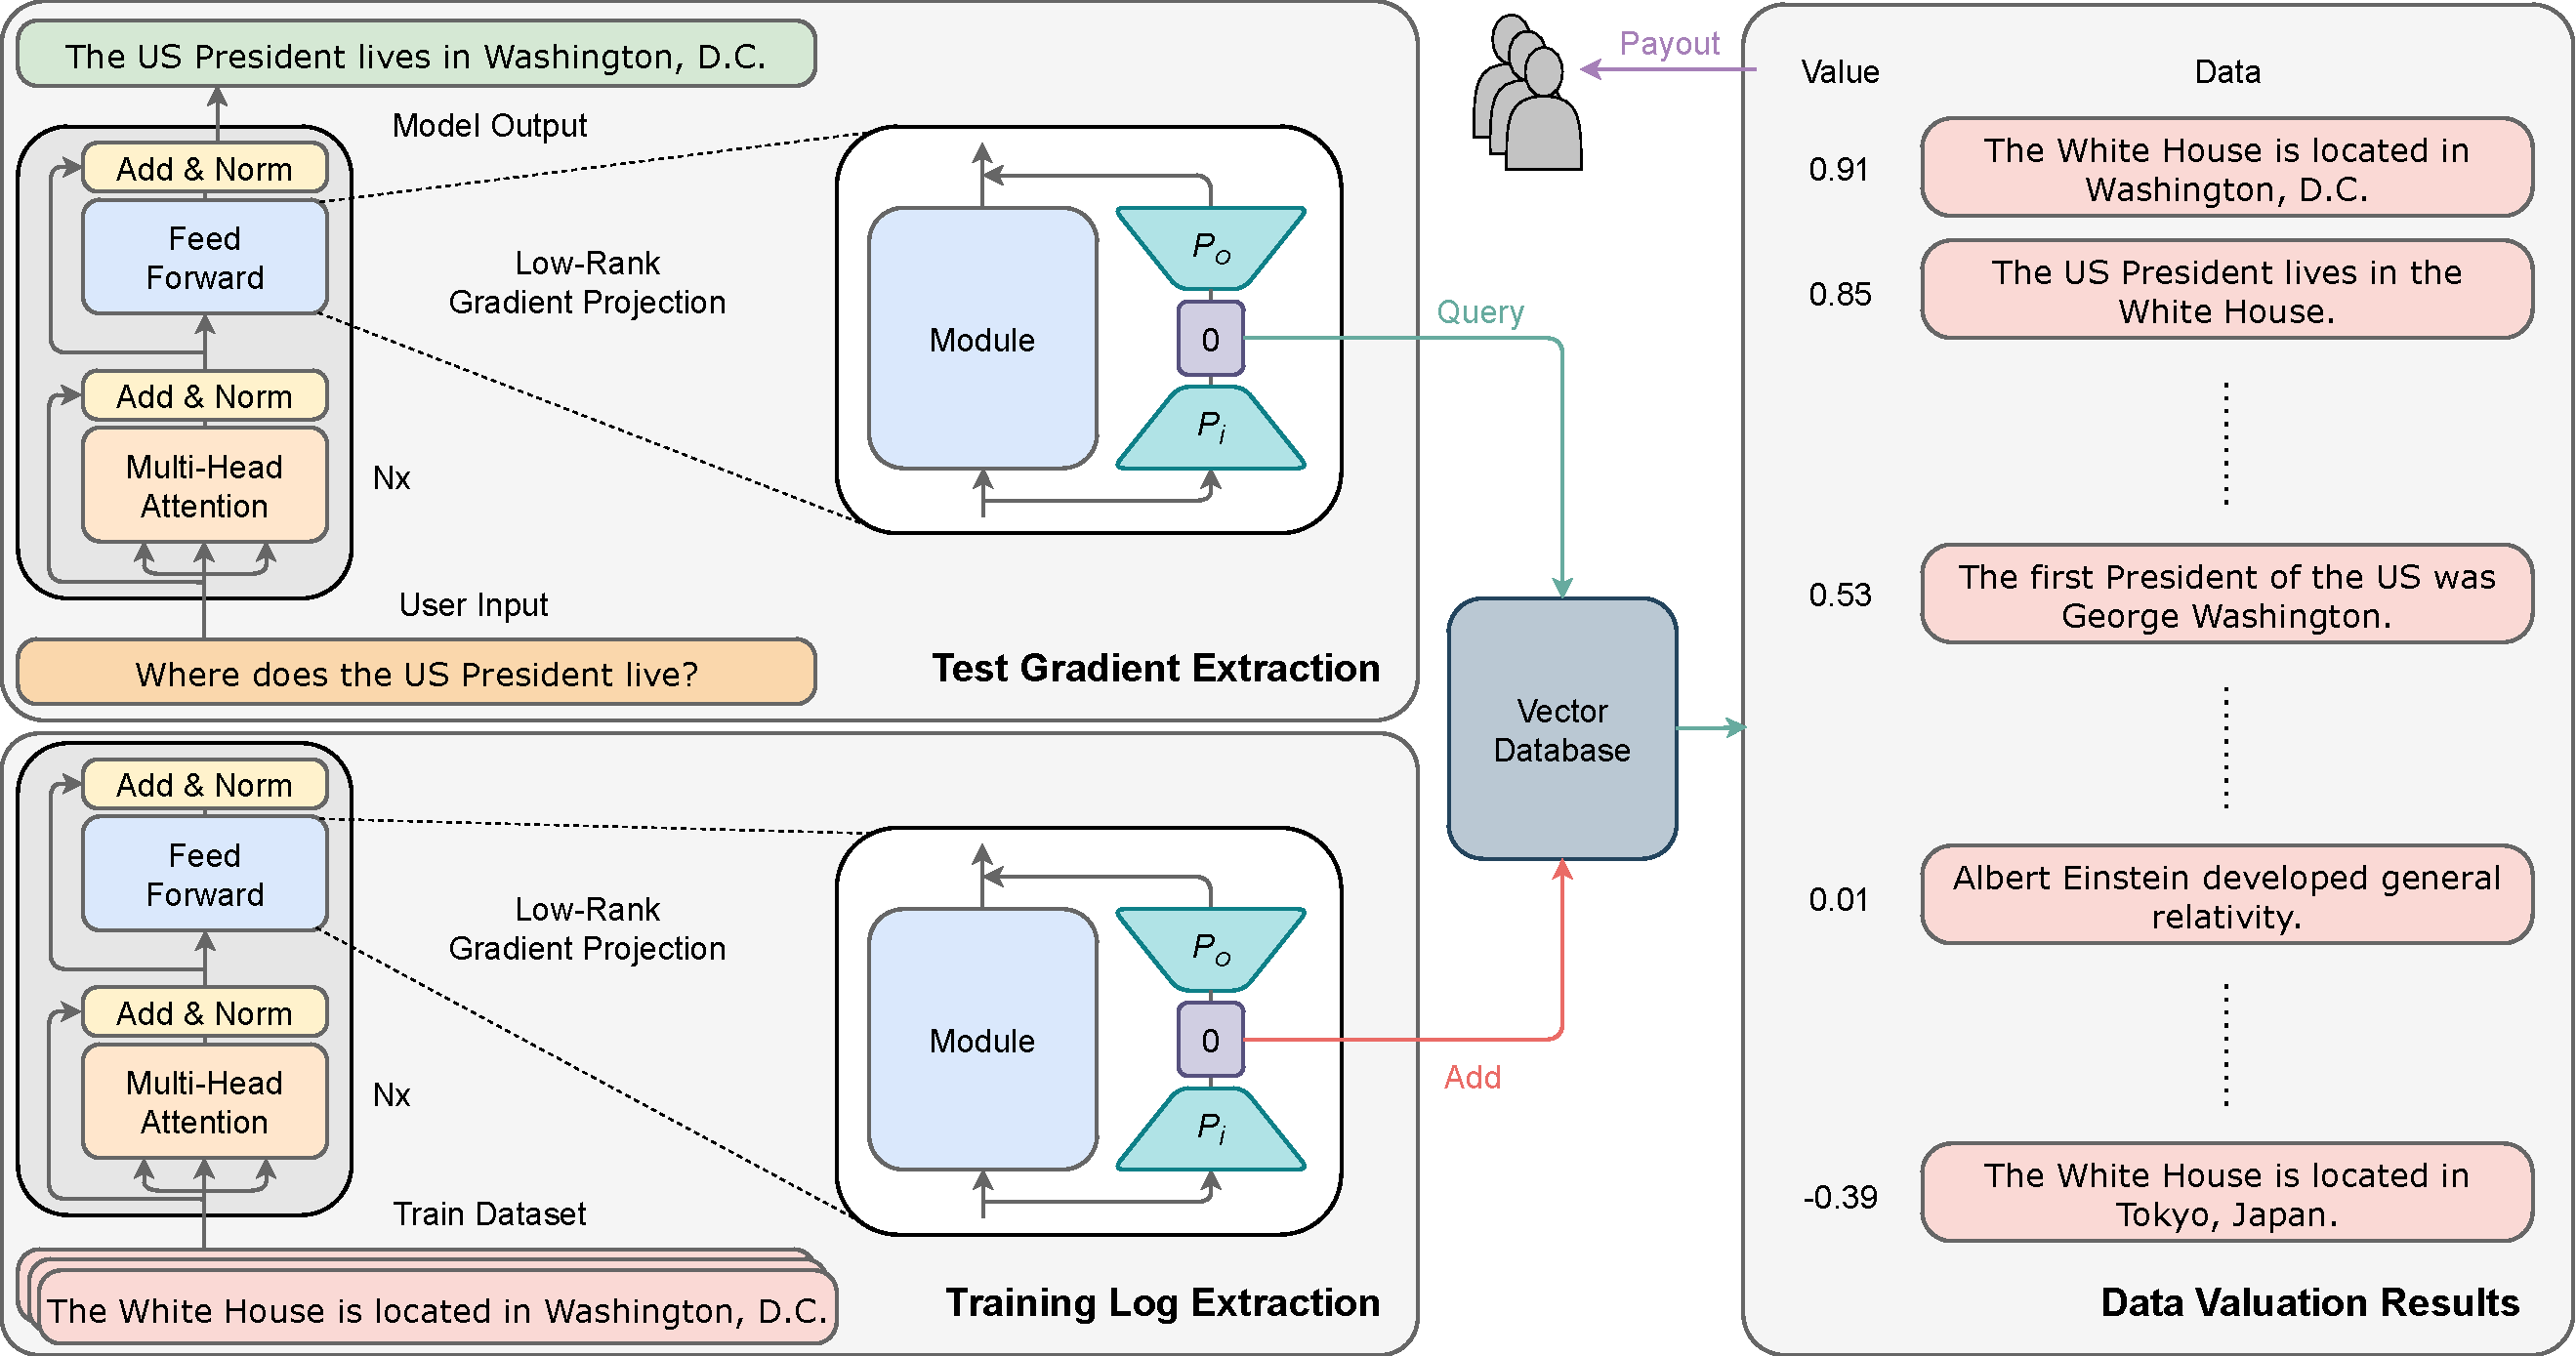
\includegraphics[width=0.94\textwidth]{figures/diagram_v7.pdf}
    \vskip -4pt
    \caption{Data valuation system architecture. \textbf{(Left Bottom)} We first extract the Hessian and gradients for all training data using efficient gradient projection \method\ and store them in a database. \textbf{(Left Top)} At test time, we similarly extract gradients and query the database. \textbf{(Right)} The database returns similarity scores with respect to training examples that can be used for data valuation/attribution.}
    \label{fig:diagram}
\end{figure}

\begin{itemize}[leftmargin=*,topsep=-2pt]
    \item Employing gradient structures in backpropagation, we develop a novel \textbf{lo}w-rank \textbf{gra}dient projection algorithm \method\ that improves space \& time complexity of gradient projection, a major scalability bottleneck in prior work~\cite{park2023trak,schioppa2022scaling}, from $O(nk)$ to $O(\sqrt{nk})$ where $n$ and $k$ are model and projection dimensions. Furthermore, \method\ directly computes projected gradients without materializing full gradients, enabling low GPU memory and high GPU utilization for improved efficiency. Lastly, we show that \method\ can be easily implemented with small add-on layers, similarly to LoRA~\cite{hu2021lora}.
    \item By interpreting a damping term in influence functions as a spectral gradient sparsification mechanism, we (1) offer a theoretical motivation of gradient projection approaches to influence functions and (2) derive a specialized PCA initialization scheme for \method.
    \item We introduce software named \software\ that (1) makes it \textit{simple} to convert existing training code into data valuation code, (2) is \textit{compatible} with various scalability tools and features in the LLM ecosystem, and (3) is \textit{extensible} to implement other data valuation or interpretability algorithms.
    \item In our data valuation experiments, \method\ demonstrates competitive accuracy against more costly baselines, while showing up to 6,500$\times$ increase in throughput and 5$\times$ reduction in GPU memory, when applied to Llama3-8B-Instruct~\cite{llama3modelcard} and the 1B-token dataset, compared to EKFAC influence \cite{grosse2023studying}, the state-of-the-art and only runnable baseline at this scale. We also observe that most valuable data identified by \method\ generally share qualitative similarities with the queried LLM output.
\end{itemize}